
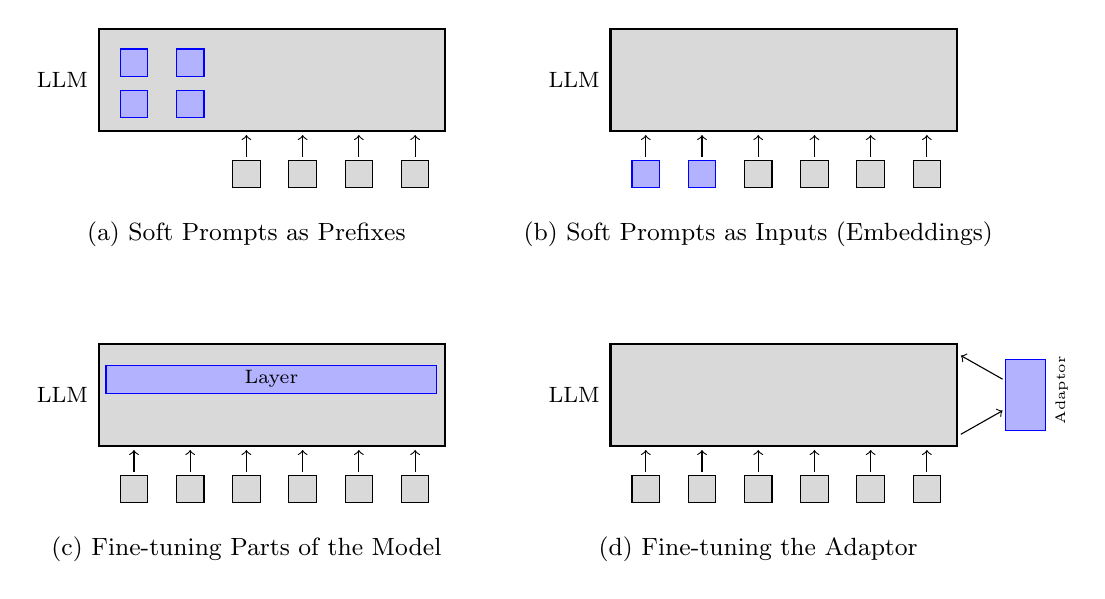
\begin{tikzpicture}

\def\ssep{0.35cm}
\def\bsep{2.0cm}

\tikzstyle{enode} = [minimum width=0.35cm,minimum height=0.35cm,inner sep=2pt,draw];
\tikzstyle{tnode} = [minimum width=4.4cm,minimum height=1.3cm,inner sep=2pt,draw,thick,fill=gray!30];

\begin{scope}

\node [enode,anchor=west,draw=white] (e0) at (0,0) {};
\node [enode,anchor=west,draw=white] (e1) at ([xshift=\ssep]e0.east) {};
\node [enode,anchor=west,fill=gray!30] (e2) at ([xshift=\ssep]e1.east) {};
\node [enode,anchor=west,fill=gray!30] (e3) at ([xshift=\ssep]e2.east) {};
\node [enode,anchor=west,fill=gray!30] (e4) at ([xshift=\ssep]e3.east) {};
\node [enode,anchor=west,fill=gray!30] (e5) at ([xshift=\ssep]e4.east) {};

\node [tnode,anchor=south west] (model) at ([yshift=\ssep,xshift=-0.8*\ssep]e0.north west) {};
\node [anchor=east] (modellabel) at ([xshift=0pt]model.west) {\footnotesize{LLM}};

\draw [->,white] ([yshift=1pt]e0.north) -- ([yshift=\ssep-1pt]e0.north);
\draw [->,white] ([yshift=1pt]e1.north) -- ([yshift=\ssep-1pt]e1.north);
\draw [->] ([yshift=1pt]e2.north) -- ([yshift=\ssep-1pt]e2.north);
\draw [->] ([yshift=1pt]e3.north) -- ([yshift=\ssep-1pt]e3.north);
\draw [->] ([yshift=1pt]e4.north) -- ([yshift=\ssep-1pt]e4.north);
\draw [->] ([yshift=1pt]e5.north) -- ([yshift=\ssep-1pt]e5.north);

\node [enode,anchor=south,draw=blue,fill=blue!30] (p0) at ([yshift=1.5*\ssep]e0.north) {};
\node [enode,anchor=south,draw=blue,fill=blue!30] (p1) at ([yshift=1.5*\ssep]e1.north) {};

\node [enode,anchor=south,draw=blue,fill=blue!30] (p01) at ([yshift=3.0*\ssep]e0.north) {};
\node [enode,anchor=south,draw=blue,fill=blue!30] (p11) at ([yshift=3.0*\ssep]e1.north) {};

\node [anchor=north] (caption) at ([yshift=-0.3cm]e2.south) {\small{(a) Soft Prompts as Prefixes}};

\end{scope}

\begin{scope}[xshift=6.5cm]

\node [enode,anchor=west,draw=blue,fill=blue!30] (e0) at (0,0) {};
\node [enode,anchor=west,draw=blue,fill=blue!30] (e1) at ([xshift=\ssep]e0.east) {};
\node [enode,anchor=west,fill=gray!30] (e2) at ([xshift=\ssep]e1.east) {};
\node [enode,anchor=west,fill=gray!30] (e3) at ([xshift=\ssep]e2.east) {};
\node [enode,anchor=west,fill=gray!30] (e4) at ([xshift=\ssep]e3.east) {};
\node [enode,anchor=west,fill=gray!30] (e5) at ([xshift=\ssep]e4.east) {};

\node [tnode,anchor=south west] (model) at ([yshift=\ssep,xshift=-0.8*\ssep]e0.north west) {};
\node [anchor=east] (modellabel) at ([xshift=0pt]model.west) {\footnotesize{LLM}};

\draw [->] ([yshift=1pt]e0.north) -- ([yshift=\ssep-1pt]e0.north);
\draw [->] ([yshift=1pt]e1.north) -- ([yshift=\ssep-1pt]e1.north);
\draw [->] ([yshift=1pt]e2.north) -- ([yshift=\ssep-1pt]e2.north);
\draw [->] ([yshift=1pt]e3.north) -- ([yshift=\ssep-1pt]e3.north);
\draw [->] ([yshift=1pt]e4.north) -- ([yshift=\ssep-1pt]e4.north);
\draw [->] ([yshift=1pt]e5.north) -- ([yshift=\ssep-1pt]e5.north);

\node [anchor=north] (caption) at ([yshift=-0.3cm]e2.south) {\small{(b) Soft Prompts as Inputs (Embeddings)}};

\end{scope}

\begin{scope}[yshift=-4cm]

\node [enode,anchor=west,fill=gray!30] (e0) at (0,0) {};
\node [enode,anchor=west,fill=gray!30] (e1) at ([xshift=\ssep]e0.east) {};
\node [enode,anchor=west,fill=gray!30] (e2) at ([xshift=\ssep]e1.east) {};
\node [enode,anchor=west,fill=gray!30] (e3) at ([xshift=\ssep]e2.east) {};
\node [enode,anchor=west,fill=gray!30] (e4) at ([xshift=\ssep]e3.east) {};
\node [enode,anchor=west,fill=gray!30] (e5) at ([xshift=\ssep]e4.east) {};

\node [tnode,anchor=south west] (model) at ([yshift=\ssep,xshift=-0.8*\ssep]e0.north west) {};
\node [anchor=east] (modellabel) at ([xshift=0pt]model.west) {\footnotesize{LLM}};

\draw [->] ([yshift=1pt]e0.north) -- ([yshift=\ssep-1pt]e0.north);
\draw [->] ([yshift=1pt]e1.north) -- ([yshift=\ssep-1pt]e1.north);
\draw [->] ([yshift=1pt]e2.north) -- ([yshift=\ssep-1pt]e2.north);
\draw [->] ([yshift=1pt]e3.north) -- ([yshift=\ssep-1pt]e3.north);
\draw [->] ([yshift=1pt]e4.north) -- ([yshift=\ssep-1pt]e4.north);
\draw [->] ([yshift=1pt]e5.north) -- ([yshift=\ssep-1pt]e5.north);

\node [anchor=west,minimum width=4.2cm,minimum height=0.3cm,fill=blue!30,draw=blue,inner sep=2pt] (layer) at ([xshift=0.1cm,yshift=0.2cm]model.west) {\scriptsize{Layer}};

\node [anchor=north] (caption) at ([yshift=-0.3cm]e2.south) {\small{(c) Fine-tuning Parts of the Model}};

\end{scope}

\begin{scope}[yshift=-4cm,xshift=6.5cm]

\node [enode,anchor=west,fill=gray!30] (e0) at (0,0) {};
\node [enode,anchor=west,fill=gray!30] (e1) at ([xshift=\ssep]e0.east) {};
\node [enode,anchor=west,fill=gray!30] (e2) at ([xshift=\ssep]e1.east) {};
\node [enode,anchor=west,fill=gray!30] (e3) at ([xshift=\ssep]e2.east) {};
\node [enode,anchor=west,fill=gray!30] (e4) at ([xshift=\ssep]e3.east) {};
\node [enode,anchor=west,fill=gray!30] (e5) at ([xshift=\ssep]e4.east) {};

\node [tnode,anchor=south west] (model) at ([yshift=\ssep,xshift=-0.8*\ssep]e0.north west) {};
\node [anchor=east] (modellabel) at ([xshift=0pt]model.west) {\footnotesize{LLM}};

\draw [->] ([yshift=1pt]e0.north) -- ([yshift=\ssep-1pt]e0.north);
\draw [->] ([yshift=1pt]e1.north) -- ([yshift=\ssep-1pt]e1.north);
\draw [->] ([yshift=1pt]e2.north) -- ([yshift=\ssep-1pt]e2.north);
\draw [->] ([yshift=1pt]e3.north) -- ([yshift=\ssep-1pt]e3.north);
\draw [->] ([yshift=1pt]e4.north) -- ([yshift=\ssep-1pt]e4.north);
\draw [->] ([yshift=1pt]e5.north) -- ([yshift=\ssep-1pt]e5.north);

\node [anchor=west,minimum width=0.5cm,minimum height=0.9cm,fill=blue!30,draw=blue] (adaptor) at ([xshift=0.6cm]model.east) {};
\node [anchor=west,rotate=90] (adaptorlabel) at ([xshift=0.2cm,yshift=-0.5cm]adaptor.east) {\tiny{Adaptor}};
\draw [<-] ([xshift=-1pt,yshift=-0.2cm]adaptor.west) -- ([xshift=1pt,yshift=-0.5cm]model.east);
\draw [->] ([xshift=-1pt,yshift=0.2cm]adaptor.west) -- ([xshift=1pt,yshift=0.5cm]model.east);

\node [anchor=north] (caption) at ([yshift=-0.3cm]e2.south) {\small{(d) Fine-tuning the Adaptor}};

\end{scope}

\end{tikzpicture}
